The sets containing the spots detected in the 
\head{} and \tail{} are referred to as \shead{} and \stail{} respectively.
For this work, we decided to map each spot to the entity with the \emph{highest commonness}, 
i.e., the highest probability $p(e|s)$ to be associated with the spot $s$ in question.

Some real query examples with annotations (spots are highlighted in bold) are provided below.
\begin{itemize}
\item \fbox{\textbf{first citizens bank} and trust \textbf{Raleigh NC}} is
annotated with the entities
\texttt{Raleigh,\_North\_Carolina} and \\ \texttt{First\_Citizens\_Bank};
% \item \fbox{\textbf{internal revenue service} de \textbf{puerto roco}} is annotated with the entities \texttt{Roco} and
% \texttt{Internal\_Revenue\_Service};
\item \fbox{\textbf{Tennessee walking horses} in \textbf{Missouri}} is annotated
with the entities  \texttt{Missouri} and  \texttt{Tennessee\_Walking\_Horse};
\item \fbox{\textbf{i love you} \textbf{remix} featuring \textbf{Jim Jones} and
\textbf{black rob}} is annotated with the entities  \texttt{I\_Love\_You,\_Man},
\texttt{Remix}, \texttt{Jim\_Jones\_(rapper)}, \texttt{Black\_Rob}.
 \end{itemize}
 
 \begin{figure}
   \centering
     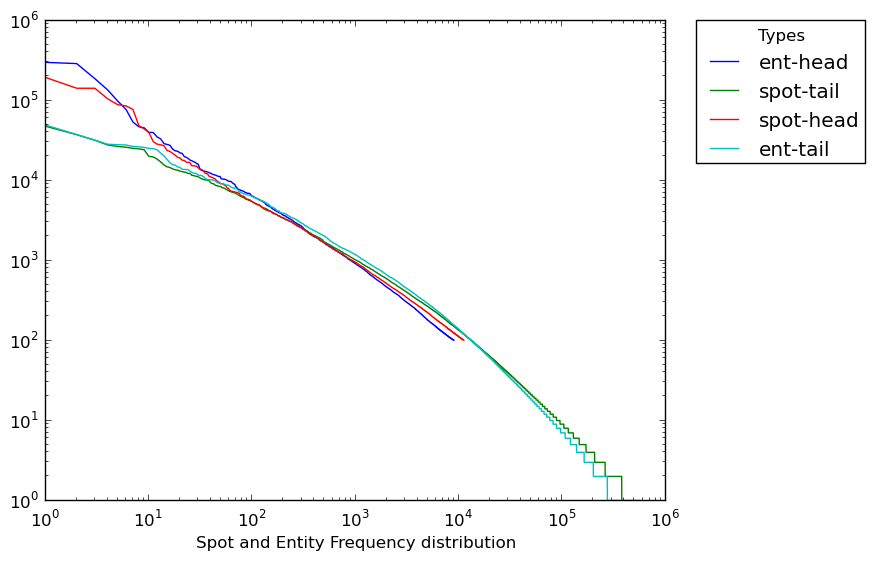
\includegraphics[width = 0.5\textwidth]{images/head-tail-ent-spot-dist.png}
 	\caption{Frequency distributions for spots and entities in \head{} (spot-head, ent-head) and \tail{} (spot-tail, ent-tail)}
 \label{img:distributions}
 \end{figure}


We denote with \ehead{} and \etail{}, the sets containing the most probable entities for the spots. To reemphasize, while \ehead{} are 
entities found in \head{}, \etail{} are found in \tail{}. 
It is worth noting that this mapping could collapse different spots on the same entity (e.g., \emph{united states} and 
\emph{Usa} will both refer to United States). Since we do not complete the
disambiguation phase, we understand that selection of
highest scored entity each time for a spot induces some bias in this analysis. We shall, in future, also take into account 
remaining spots and terms in the query for entity disambiguation. 

There are $11,152$ ($|$\shead{}$|$)  distinct spots and $8,949$ ($|$\ehead{}$|$) distinct 
entities in the head. In the tail, the system identifies $550,953$ ($|$\stail{}$|$) distinct spots and 
$379,342$ ($|$\etail{}$|$) distinct entities. It  is also interesting to note the size of the 
intersections: \mbox{$|$\shead{}$\cap$\stail{}$|=11,027$}  $|$\ehead{}$\cap$\etail{}$| = 8,888$,
this means that almost all the spots and entities in the head appear in the tail. 

Figure~\ref{img:distributions} shows the frequency distribution of both head and tail spots as well as head and tail entities:
it is interesting to note that while queries in head and tail follow totally different distributions, when we look at their 
spots/entities, the distributions are similar. In particular, as expected, head spots and head entities 
follow a similar distribution, as well as the spots and entities in the tail. 


\begin{figure*}[t]
	\footnotesize
	\centering
\begin{tabular}{lc|lc|lc|lc}
\toprule
\multicolumn{4}{c}{\head{}} & \multicolumn{4}{c}{\tail{}}\\
\multicolumn{2}{c}{\shead{}} & \multicolumn{2}{c}{\ehead{}} & \multicolumn{2}{c}{\stail{}} & \multicolumn{2}{c}{\etail{}}\\
\midrule
google         & 342,602  &  Google  		   & 349,337  &  florida 	 &	47,718	&	Florida 		& 49,366 \\
myspace        & 194,093  &  Yahoo\!  		   & 299,718  &  texas  	 &	 37,388  &   Texas   		& 37,526 \\
yahoo          & 142,361  &  Myspace 		   & 289,353  &  ohio    	 &	31,861   &   Ohio    		& 31,905 \\			
ebay           & 142,257  &   EBay   		   & 187,633  &  edu     	 &	26,641   &   New\_York        & 28,396 \\
yahoo.com      & 104,696  &  MapQuest          & 135,179  &  state   	 &	26,066   &   .edu    		& 26,642 \\
mapquest       & 88,617   &  Google\_Search     & 98,112   &  california  &   25,233  &   U.S.\_state      & 26,392 \\
google com     & 85,670   &  Hotmail           & 53,925   &  new york    &   24,865  &   California      & 25,859 \\
my space       & 48,401   &	  Bank\_of\_America  & 46,922   &  hotel   	 &	20,018   &   Real\_estate     & 25,232 \\
www.yahoo.com  & 44,198   &  Craigslist        & 45,586   &  real estate &   19,702  &   Myspace 		& 24,998 \\
internet       & 39,865   &  Ask.com           & 39,873   &  myspace 	 &	18,533   &   Floruit 		& 24,207 \\
ebay com       & 30,652   &  Internet          & 39,865   &  restaurant  &  17,065   &   Restaurant      & 21,996 \\
hotmail.com    & 28,492   &  Pornography       & 35,089   &  michigan    &   15,635  &   Hotel   		& 20,289 \\
map quest      & 27,949   &  Tattoo            & 33,113   &  new jersey  &   14,813  &   Nudity  		& 18,245 \\
craigslist     & 27,222   &  American\_Idol     & 28,890   &  georgia 	 &	14,525   &   United\_States   & 16,680 \\
american idol  & 23,665   &  Yahoo!\_Mail       & 28,238   &  black   	 &	13,921   &   Michigan        & 15,763 \\
\bottomrule
\end{tabular}
\label{tab:top-frequent}
\caption{Most 15 frequent spots and entities detected in the head (\shead{}, \ehead{}) and in the tail (\stail{}, \etail{})}
\end{figure*}

Do the most frequent entities in \ehead{} and \etail{} overlap? Not so much: we sorted the entities
based on their total frequency within all the queries of \head{} and \tail{} to compare
the ranked lists at different cutoffs ($50$, $100$, $500$, $5000$). We then computed the Jaccard distance
between the ranked lists, obtaining $0.25$ when considering the most $5000$ most frequent entities,
and $0.21$ considering the most frequent spots. At smaller cutoffs the Jaccard was considerably small, 
when we consider the top $50$ entities in head and tail, Jaccard equals to $0.05$. 
Table~\ref{tab:top-frequent} lists the most frequent entities and spots in both head and the tail. 
It is interesting to observe that, while the head contains several navigational entities (google, yahoo etc.), the 
tail contains several US countries.
% \todo{introduce \shead{} \stail{} \ehead{} \etail{} and
% \begin{itemize}
% 	\item comment table with commonness and link probability + top entities/spots
% 	\item put total numbers
% 	\item put global distribution
% \end{itemize}
% }

%\todo{introduce the comparison between tail and head }

%\todo{describe Figure~\ref{img:headTailEntPercent}}

%\todo{explain how head tail ratio is computed, present and comment the graph }

%\todo{conclusions and future works (e.g, use a modern query log, improve entity linking on queries, considering sessions)}

% diego put this in the intro if there's space
% Tail queries have been often mapped to the head \cite{} by using bag-of-word representations.
% Lately they have also been linked with the head queries through entities. However, in this work
% we attempt to study the extent to which the entities in the tail queries can be linked to entities
% in the head queries. It is important to know how much will entity linking at tail benefit query mining.
% We shall, from now on refer to entities in head queries as `head entity'
% and entities occuring in the tail as `tail entity'.

\begin{figure}
\label{img:headTailEntPercent}
  \centering
    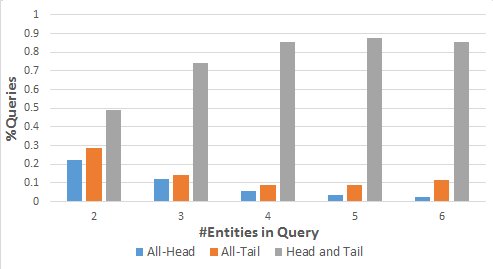
\includegraphics[width = 0.45\textwidth]{images/entity-head-tail-count.png}
	\caption{Percentage of tail queries with only head, only tail or both entities}
\end{figure}
 
% We begin by analyzing the volume of entities found in the tail. Of X unique tail queries,
% 63.2\% contain atleast one entity.
%Of queries containing more than one entity, 86.2\% queries contain atleast one head entity. 
%Once, the queries in the tail are tagged with entities, 
There are several queries in the log with multiple entities. 
%The number of entities and corresponding query distribution is shown in Table \ref{table:entityQueryDist}. 
On average tail queries tend to have more entities than head. 
To investigate whether tail queries inquire about entities in the head, we analyze percentage of tail queries containing 
only head entities, only tail entities ($\in$ \etail{} $\setminus$ \ehead{}) or both. Figure \ref{img:headTailEntPercent} 
depicts the percentage of queries with respect to number of entities in the query. 
One can clearly see that a large percentage of tail queries contains both head and tail entities. 
Moreover, this percentage gradually rises with the number of entities in the query. 
This indicates that in longer queries people look for connections among popular entities and rare entities. 
%Next we analyze what fraction of queries contain only head entities, only \emph{tail entities}, i.e., entities 
%that appear \emph{only} in the tail ($\in$ \etail{} $\setminus$ \ehead{})
%or both head and tail entities.

%\begin{table}
%\caption{Number of Entities vs Head and Tail Queries}	
%\label{table:entityQueryDist}
%\centering
%\begin{tabular}{|l|l|l|}
%\hline
%\#Entities	&	Tail	&	Head	\\ \hline
%0	&	2844620	&	5976	\\ \hline
%1	&	2622873	&	12904	\\ \hline
%2	&	1731256	&	1039	\\ \hline
%3	&	457946	&	32	\\ \hline
%4	&	74125	&	1	\\ \hline
%5	&	10757	&	1	\\ \hline
%6	&	2416	&	0	\\ \hline
%>6	&	2613	&	0	\\ \hline
%\end{tabular}
%\end{table}


% Provided that such a large percentage of tail queries contain both head and tail entities, it
% will be useful to see the ratio of head entities to tail entities in these queries. Especially,
% for queries with more than 2 entities, it would be interesting to see whether head queries occur more
% than tail queries or vice versa. Table \ref{table:entDist} shows the number of entities in the query,
% number of such queries and the average head to tail entity ratio of these queries.
% Although, there are queries with more than 6 entities, they are too few to draw any significant
% conclusions. PLEASE ADD > 6 RESULTS AS WELL.
% %1.no of queries with head and tail ent
% %2.Head and tail entity histogram for queries with more than 1 ent
% Head to Tail entity ratio is calculated by dividing number of head entities with number of
% tail entities in the query, i.e. $E_{head}/E_{tail}$. It is interesting to note that queries with
% more entities have almost equal number of head and tail entities. Few query examples are provided in
% Table \ref{table:queriesWithEnt}. The entities are in bold. What is interesting is the nature of tail
% entities that co-occur with the head.
%
% \begin{table}
% \caption{\#Entities vs \#Queries}
% \label{table:entDist}
% \centering
% \begin{tabular}{|l|l|l|}
% \hline
% \#Entities & \#Queries & Head Tail Ratio \\ \hline
% 1 & 2622873 & NA \\ \hline
% 2 & 1731256 & 0.48 \\ \hline
% 3 & 457946  & 0.91 \\ \hline
% 4 & 74125 & 1.09  \\ \hline
% 5 & 10757 & 1.07 \\ \hline
% 6 & 2416  & 0.97 \\ \hline
% \end{tabular}
% \end{table}
%
% %The table clearly shows that for every tail entity there is a head entity in the query.
%
% Figure \ref{img:headTailEntBreakup} shows the percentage of queries for each ratio

% \begin{table*}
% \caption{Example queries with head and tail entities}
% \label{table:queriesWithEnt}
% \centering
% \begin{tabular}{|l|l|l|l|}
% \hline
% Query &  Head Entities & Tail Entities \\ \hline
% \textbf{first citizens bank} and trust \textbf{raleigh nc} & Raleigh,\_North\_Carolina & First\_Citizens\_Bank  \\ \hline
% \textbf{internal revenue service} de \textbf{puerto roco} & Roco & Internal\_Revenue\_Service \\ \hline
% \textbf{seafood sticks} \textbf{celery} \textbf{cheese} \textbf{egg} \textbf{casserole} \textbf{asian recipes} & Crab\_stick, Casserole, Celery & Race\_and\_ethnicity\_in\_the\_United\_States\_Census, Egg, Cheese \\ \hline
%
% \textbf{tennessee walking horses} in \textbf{missouri} sale & Missouri & Tennessee\_Walking\_Horse \\ \hline
% \textbf{i love you} \textbf{remix} featuring \textbf{jim jones} and \textbf{black rob} & I\_Love\_You,\_Man, Remix & Jim\_Jones\_(rapper), Black\_Rob \\ \hline
% \end{tabular}
% \end{table*}

% \begin{figure}[t]
% \label{img:headTailEntBreakup}
% \caption{\%Queries vs Head to Tail Entity Ratio}
%   \centering
%     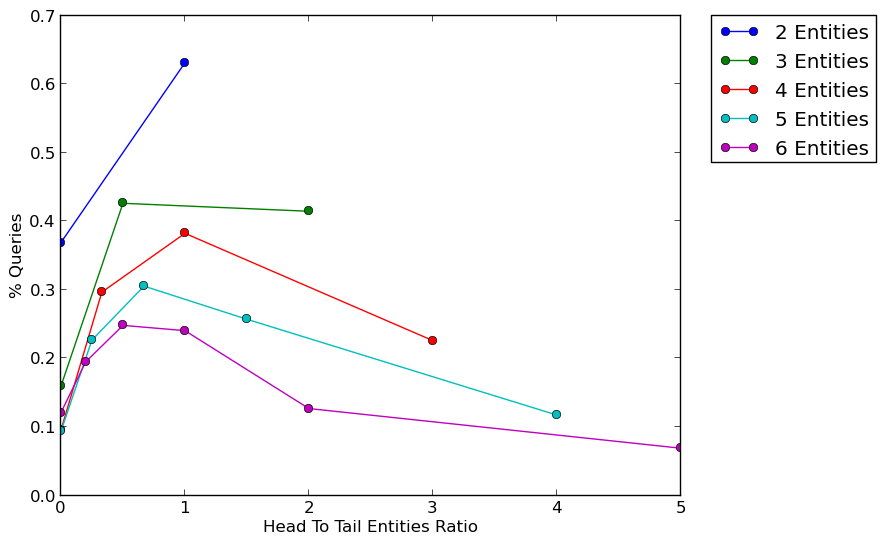
\includegraphics[width = 0.45\textwidth]{images/entity-head-query-ratio-dist.png}
% \end{figure}

%Head entity popularity
% Given that there would several head entities, not all of them will be equally popular.
% Here, popularity of the entity refers to the scope of that entity, how many entities does
% it co-occur with, or how common is that entity.
% Figure \ref{img:headEntDist} shows the frequency distribution of head entities in the
% head queries. That is, how frequently does a head entity occur in popular queries.
% To aggregate statistics for the tail, we divide head entities into 7 buckets, each bucket
% spanning 20\% of entities. This results in X popular entities being in 0-20\% range, Y
% entities in 20-40\% range, so on and so forth.


% \begin{figure}[t]
% \label{img:headEntDist}
% \caption{Cumulative Distribution of Entity Frequency in Head Queries}
%   \centering
%     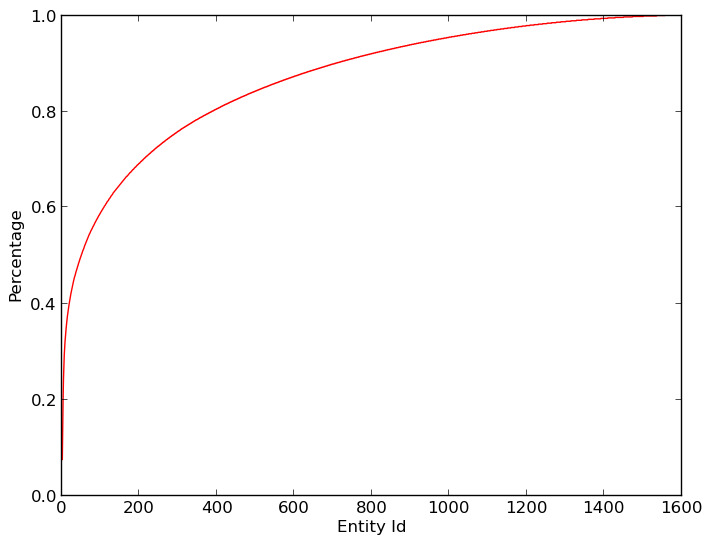
\includegraphics[width = 0.45\textwidth]{images/entity-head-dist.png}
% \end{figure}



% The co-occurrance of tail entities with head entities of different grades is shown in
% Figure \ref{img:headEntDistInTail}. The figure clearly indicates that
% WRITE ABOUT THE PLOT HERE

 
% \begin{table}
% \caption{Queries per Popularity of Head Entity}
% \label{table:headEntQueryDist}
% \centering
% \begin{tabular}{|l|l|l|}
% \hline
% Popularity & \#Entities & Queries \\ \hline
% 0-20\% & 3 & 14851 \\ \hline
% 20-40\% & 18  & 57611.0 \\ \hline
% 40-60\% & 95 & 149733.0 \\ \hline
% 60-80\% & 287 & 299561.0 \\ \hline
% 80-95\% & 560 & 569271.0 \\ \hline
% 95-97\% & 236 & 298498.0 \\ \hline
% 97-100\% & 349 & 854345. 0  \\ \hline
% \end{tabular}
% \end{table}


% \begin{figure}[t]
% \label{img:headRankInTail}
% \caption{\%Queries vs Rank of Head Entities}
%   \centering
%     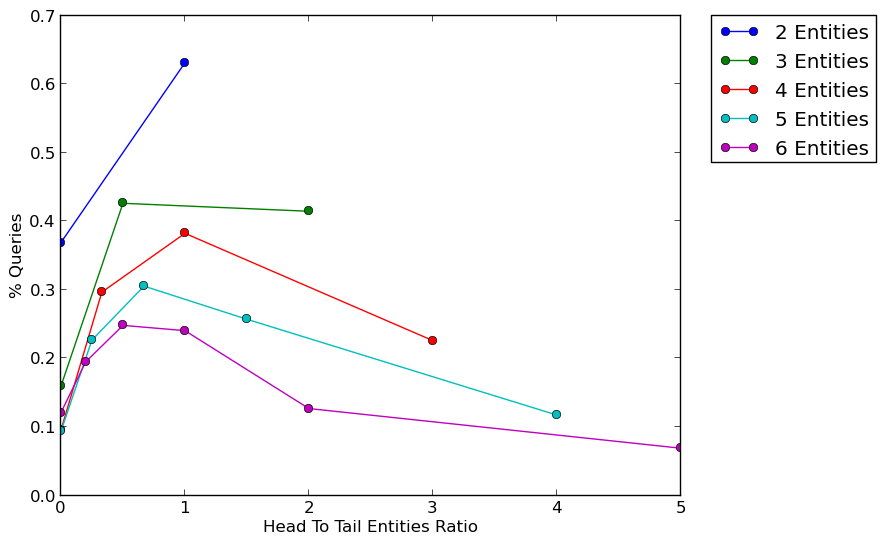
\includegraphics[width = 0.45\textwidth]{images/entity-head-query-ratio-dist.png}
% \end{figure}

%In entity analysis of Aol query logs we calculate the following:
%\begin{itemize}
%\item No of queries with entities from the head or tail
%\item Frequency distribution of entities in head and tail
%\item Head and tail entity distribution in queries
%\end{itemize}
% \begin{tabular}{ccccc}
% \toprule
% link probability & commonness & $k$ & $J^{spot}_k$ & $J^{top entity}_k$ \\
% \midrule
% \multirow{6}{*}{$0.3$} &  \multirow{3}{*}{$0.3$} & $50$ &  $0.01$  &   $0.03$  \\
% 					 &						   & $500$ 	&  $0.11$  &   $0.14$  \\
% 					 &						   & $5,000$ & $0.21$   &  $0.25$    \\
% \cline{2-5}
% 					 &	\multirow{3}{*}{$0.7$}  & $50$      & $0.01$   &   $0.03$ \\
% 					 &						   & $500$   	& $0.11$   &   $0.14$  \\
% 					 &						   & $5,000$ 	& $0.21$   &   $0.27$    \\
%
% \midrule
% \multirow{6}{*}{$0.7$} &  \multirow{3}{*}{$0.3$}   & $50$  & $0.05$   &   $0.06$  \\
% 					 &						   & $500$ 	   &   $0.11$   &    $0.13$  \\
% 					 &						   & $5,000$   &   $0.22$   &  $0.26$  \\
% \cline{2-5}
%
% 					 &	\multirow{3}{*}{$0.7$}  & $50$   &  $0.05$   &  $0.06$  \\
% 					 &						   & $500$   &  $0.11$   &   $0.15$   \\
% 					 &						   & $5,000$ &  $0.22$   &   $0.28$  \\
% \bottomrule
% \end{tabular}
